\chapter{First Contribution}
\label{chap:chapter3}
We have studied various anomaly detection techniques deployed by cloud service providers for their services. The study from our side for various cloud service providers for anomaly detection is our first contribution for the project. In this study we took three major service providers Microsoft,Amazon and Google.\\
\section{How Microsoft detects anomaly in azure}
Microsoft uses a technology called security centre\cite{microsf41} in its cloud environments.To detect threats and reduce false positives Security Centre collects data from Azure resources and network and then applies a lot of  machine learning and big data algorithms to detect threat.These techniques as more advance than normal signature based anomaly detection techniques.It is impossible to manually identify the attack and predict the attack when it might happen.So the Microsoft \\ Security Centre uses following technologies\\\\
\textbf{Intelligent threat intelligence} \newline It looks for bad actors by using the information obtained via Microsoft Products and services,Microsoft Digital Crimes Unit and Microsoft Security Response Centre along with external feeds.Microsoft has an immense amount of global threat intelligence. Telemetry flows in from multiple sources, such as Azure, Office 365, Microsoft CRM online, Microsoft Dynamics AX, outlook.com, MSN.com, the Microsoft Digital Crimes Unit (DCU), and Microsoft Security Response Center (MSRC). Researchers also receive threat intelligence information that is shared among major cloud service providers and feeds from other third parties. Azure Security Center can use this information to alert you to threats from known bad actors.\newline \newline
\textbf{Behavioral analytics} \\ Behavioral analytics is a technique that analyzes and compares data to a collection of known patterns. However, these patterns are not simple signatures. They are determined through complex machine learning algorithms that are applied to massive datasets. They are also determined through careful analysis of malicious behaviors by expert analysts. Azure Security Center can use behavioral analytics to identify compromised resources based on analysis of virtual machine logs, virtual network device logs, fabric logs, crash dumps, and other sources.
In addition, there's correlation with other signals to check for supporting evidence of a widespread campaign. This correlation helps to identify events that are consistent with established indicators of compromise.\newline \newline
\textbf{Anomaly detection}\\It uses statistical techniques to build a historical data which is based on usage patterns and any deviation from normal alerts those deviations and it creates a baseline which if confirms to a potential attack vector then the particular usage is detected as an anomaly and in turn thus could be a security event.\newline\newline
Security Centre in Azure also works with connected partner solutions, like firewall and endpoint protection solutions. Microsoft uses \textbf{Fusion Analytics} \cite{mslinks2} as the backbone of Security Centre's anomaly detection system.Fusion works by looking at various kind of alerts generated in Microsoft Azure ecosystem and then it tries to find  pattern which could reveal attack progression indicating what should be next course of action.
\section{How Amazon finds anomalies in AWS}
Amazon uses a technology called guard duty\cite{amazon2}.It is a threat detection service which continuously monitors for bad behavior and protects aws accounts and workloads.In the cloud collection and aggregation of  network activities is simplified, but it can be time consuming for security teams to continuously analyze event log data for potential threats. With the help of GuardDuty now you have an intelligent and cost effective solution to for threat detection in AWS cloud. This technology uses machine learning, anomaly detection, and integrated threat intelligence to identify and prioritize potential threats. GuardDuty analyzes tens of billions of events across multiple AWS data sources, such as AWS CloudTrail, Amazon VPC Flow Logs, and DNS logs. With a few clicks in the AWS Management Console, GuardDuty can be enabled with no software or hardware to deploy or maintain. By integrating with AWS CloudWatch Events, GuardDuty alerts are actionable, easy to aggregate across multiple accounts, and straightforward to push into existing event management and workflow systems.
\section{How Google finds anomalies in GCP cloud }
Google uses an open source library Forseti\cite{google31} which can\\
\begin{itemize}
    \item Detect unusual firewall behaviors between snapshots.
    \item Alert users to any unusual behaviors and provide a comparison with expected behaviors.
    \item Provide potential remediation steps.
\end{itemize}

The key elements for this technology are firewall rules.Firewall rules can be inbound or outbound.A firewall rule can either allow traffic based on IP address or ports.Firewall rules are applied to those instances which are associated with the user who has created his cloud in GCP setup.
The figure below shows the technical architecture as how this has been implemented in GCP \newline


\begin{figure}[h]
    \centering
    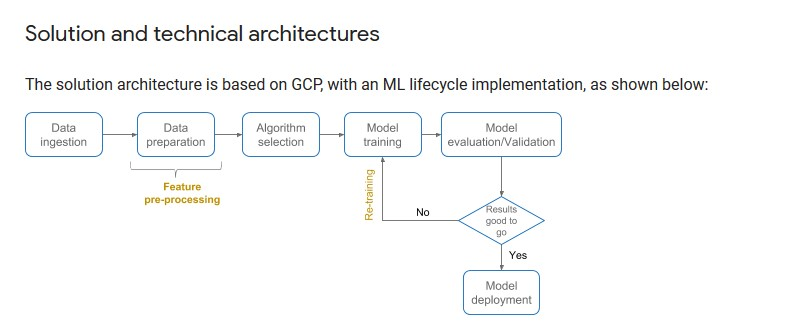
\includegraphics{texfiles/images/gcp_security_model1.jpg}
    \caption{GCP Anomaly Detection}
    \label{fig:GCP Anomaly Detection}
\end{figure}


